\section{Iteración III}
\subsection{Resumen}
En ésta iteración se realizó el frontend del login de ARF así como el backend para los módulos ``LOGIN", ``REGISTRAR CUENTA" y ``GUARDAR ESCENARIO" de acuerdo a la arquitectura descrita en la figura 4.25. \par

%\subsection{Diagramación}
\subsection{Desarrollo}
El desarrollo de los módulos de backend mencionados se realizó sobre Lambdas de AWS. Cada módulo tiene su propia función. El objetivo de hacerlo de esta forma es brindarle escalabilidad al sistema pues el desarrollo se logra de forma modular.\par
Cada uno de estos módulos es accesible a través del protocolo HTTP gracias a la API Gateway. La API Gateway es un módulo de Amazon Web Services que permite que los recursos de AWS sean accesibles desde el exterior, en éste caso, permite que la aplicación en Android pueda acceder a éstas funciones con una simple petición.\par
Las Lambdas y la API Gateway están configuradas para que a través del método POST y el formato JSON la aplicación pueda comunicarse y usar las funciones almacenadas en la nube.\par
El desarrollo de cada función en la nube se realizó con NodeJS v8.10.0. A continuación se describe cada módulo. \par
\subsubsection{Login}
Se encarga de la funcionalidad del login de la aplicación. En la figura 4.29 se puede observar el diagrama del proceso de login.\par
\begin{figure}[h!]
	\centering
	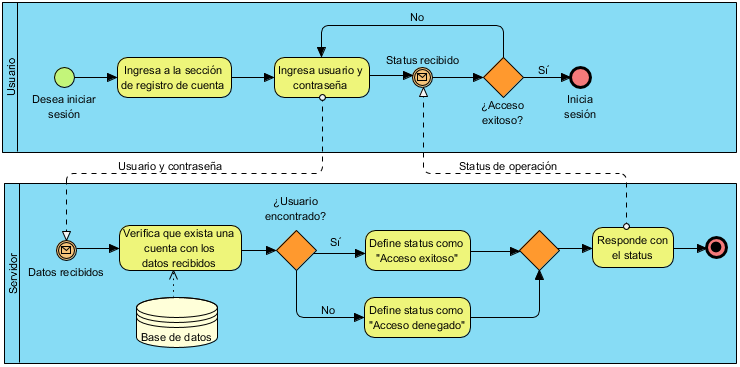
\includegraphics[width=15cm,height=9cm]{imagenes/desarrollo/diagramas/BPMN_LOGIN.png}
	\caption{Diagrama de proceso de Login.}
	\label{fig:loginsuccess}
\end{figure}
Ésta función recibe dos parámetros: usuario y contraseña. Posteriormente inicia un primer proceso de validación, el cual consiste en la obtención del hash criptográfico de la contraseña. Ese hash junto con el usuario es buscado en una base de datos relacional donde se encuentran los usuarios, esta base de datos está almacenada en Amazon RDS, que tiene un motor MySQL 5.5. Si encuentra alguna coincidencia entonces significa que el usuario existe.\par Así, la función regresa en formato JSON el usuario junto a su hash para que la aplicación valide el inicio de sesión. \par

Por otro lado si los datos ingresados son incorrectos, la función responde con un código de error, que es manipulado por la aplicación para indicar que los datos de inicio de sesión son incorrectos.

\subsubsection{Registro}
Ésta función se encarga de registrar un nuevo usuario en la base de datos para que posteriormente pueda iniciar sesión en la aplicación. El modelado de este proceso se puede apreciar en la figura 4.32. \par
\begin{figure}[h!]
	\centering
	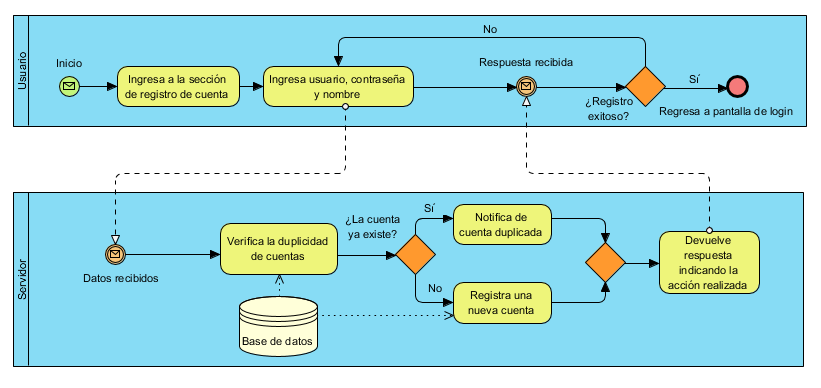
\includegraphics[width=15cm,height=7cm]{imagenes/desarrollo/diagramas/BPMN_REGISTRAR_CUENTA.png}
	\caption{Proceso de registro de nuevo usuario.}
	\label{fig:regsuccess}
\end{figure}


Funciona de manera similar a la Lambda del Login. Recibe tres parámetros en formato JSON a través de un request con método POST, estos parámetros son: nombre de usuario, contraseña y primer nombre. \par
Esta función se encarga de tomar estos datos y registrar un nuevo usuario con ellos. La contraseña que se guarda en la base de datos es el hash criptográfico con SHA-512, la cual será usada en el primero proceso de validación del inicio de sesión. En la figura 4.33 se observa el flujo de información para esta función.
\begin{figure}[h!]
	\centering
	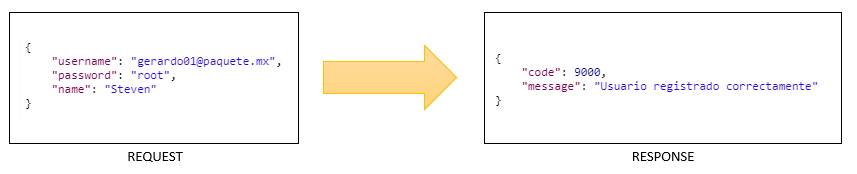
\includegraphics[width=15cm,height=3.5cm]{imagenes/desarrollo/arquitectura/REGISTER_SUCCESS.png}
	\caption{Flujo de información de registro de usuario.}
	\label{fig:regsuccess}
\end{figure}
\par

\subsubsection{Guardar escenario}
El objetivo de ésta función es poder almacenar los escenarios que vayan generando los usuarios para que después puedan ser visualizados desde la aplicación. En la figura 4.34 se puede apreciar el modelado del proceso de almacenamiento de escenario. \par
\begin{figure}[h!]
	\centering
	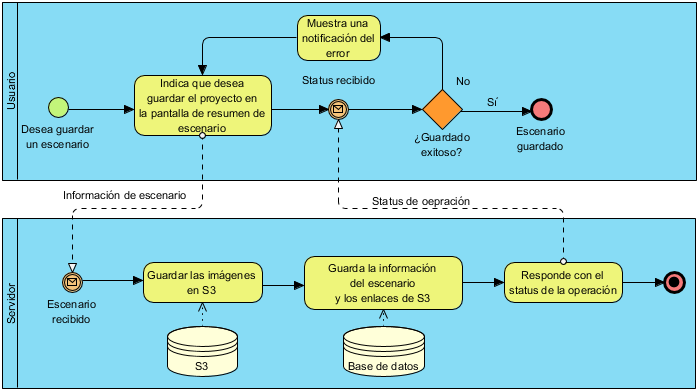
\includegraphics[width=13cm,height=7cm]{imagenes/desarrollo/diagramas/BPMN_STORESC.png}
	\caption{Proceso de guardado de escenario.}
	\label{fig:regsuccess}
\end{figure}

La función recibe como parámetros el id del usuario al que se va a asociar el escenario, el nombre del escenario y un array de imágenes en formato \textbf{Base64}. una vez recibidos estos atributos, la función se encarga de convertir las imágenes en formato binario para después guardarlas en un Bucket de AWS S3 (Simple Storage Service) que no es más que un contenedor de archivos. Una vez guardadas las imágenes en el Bucket, se obtienen los nombres y las URL de las imágenes guardadas. Los nombres sirven para guardar el escenario en una base de datos, y posteriormente poder recuperarlos del Bucket a través del nombre. Las URL de las imágenes se envían con el objetivo de poder visualizar el escenario guardado en el dispositivo móvil obteniendo las imágenes directamente del almacenamiento en la nube. El proceso de devolver las URL de las imágenes será implementado también en la función de ``VER ESCENARIO" con el objetivo de hacer que la respuesta a la petición sea más ligera, y con ello más rápida.